\newpage
\section{Test Results} \label{sec:apptestres}

\subsection{Test 28: Pump Operations}
\label{sec:test28result}

The pump was connected via crocodile connections to a power supply set to 24 V. The power supply was then switched on and the current was read off. This set-up can be seen in Figure \ref{fig:pump-testing}.

It was found that when the power supply was switched on the current went up to 600 mA for less than one second. It then settled to 250 mA. By covering the air intake, simulating air intake from a lower pressure, the current drops to 200 mA. By covering the air output, simulating pushing air into a higher pressure, the current rises to 400 mA.

Therefore the power for each of these conditions is 14.4 W at turn on, 6 W in normal use, 4.8 W when sucking from low pressure, 9.6 W when pushing to high pressure.


\begin{figure}[H]
    \begin{align*}
        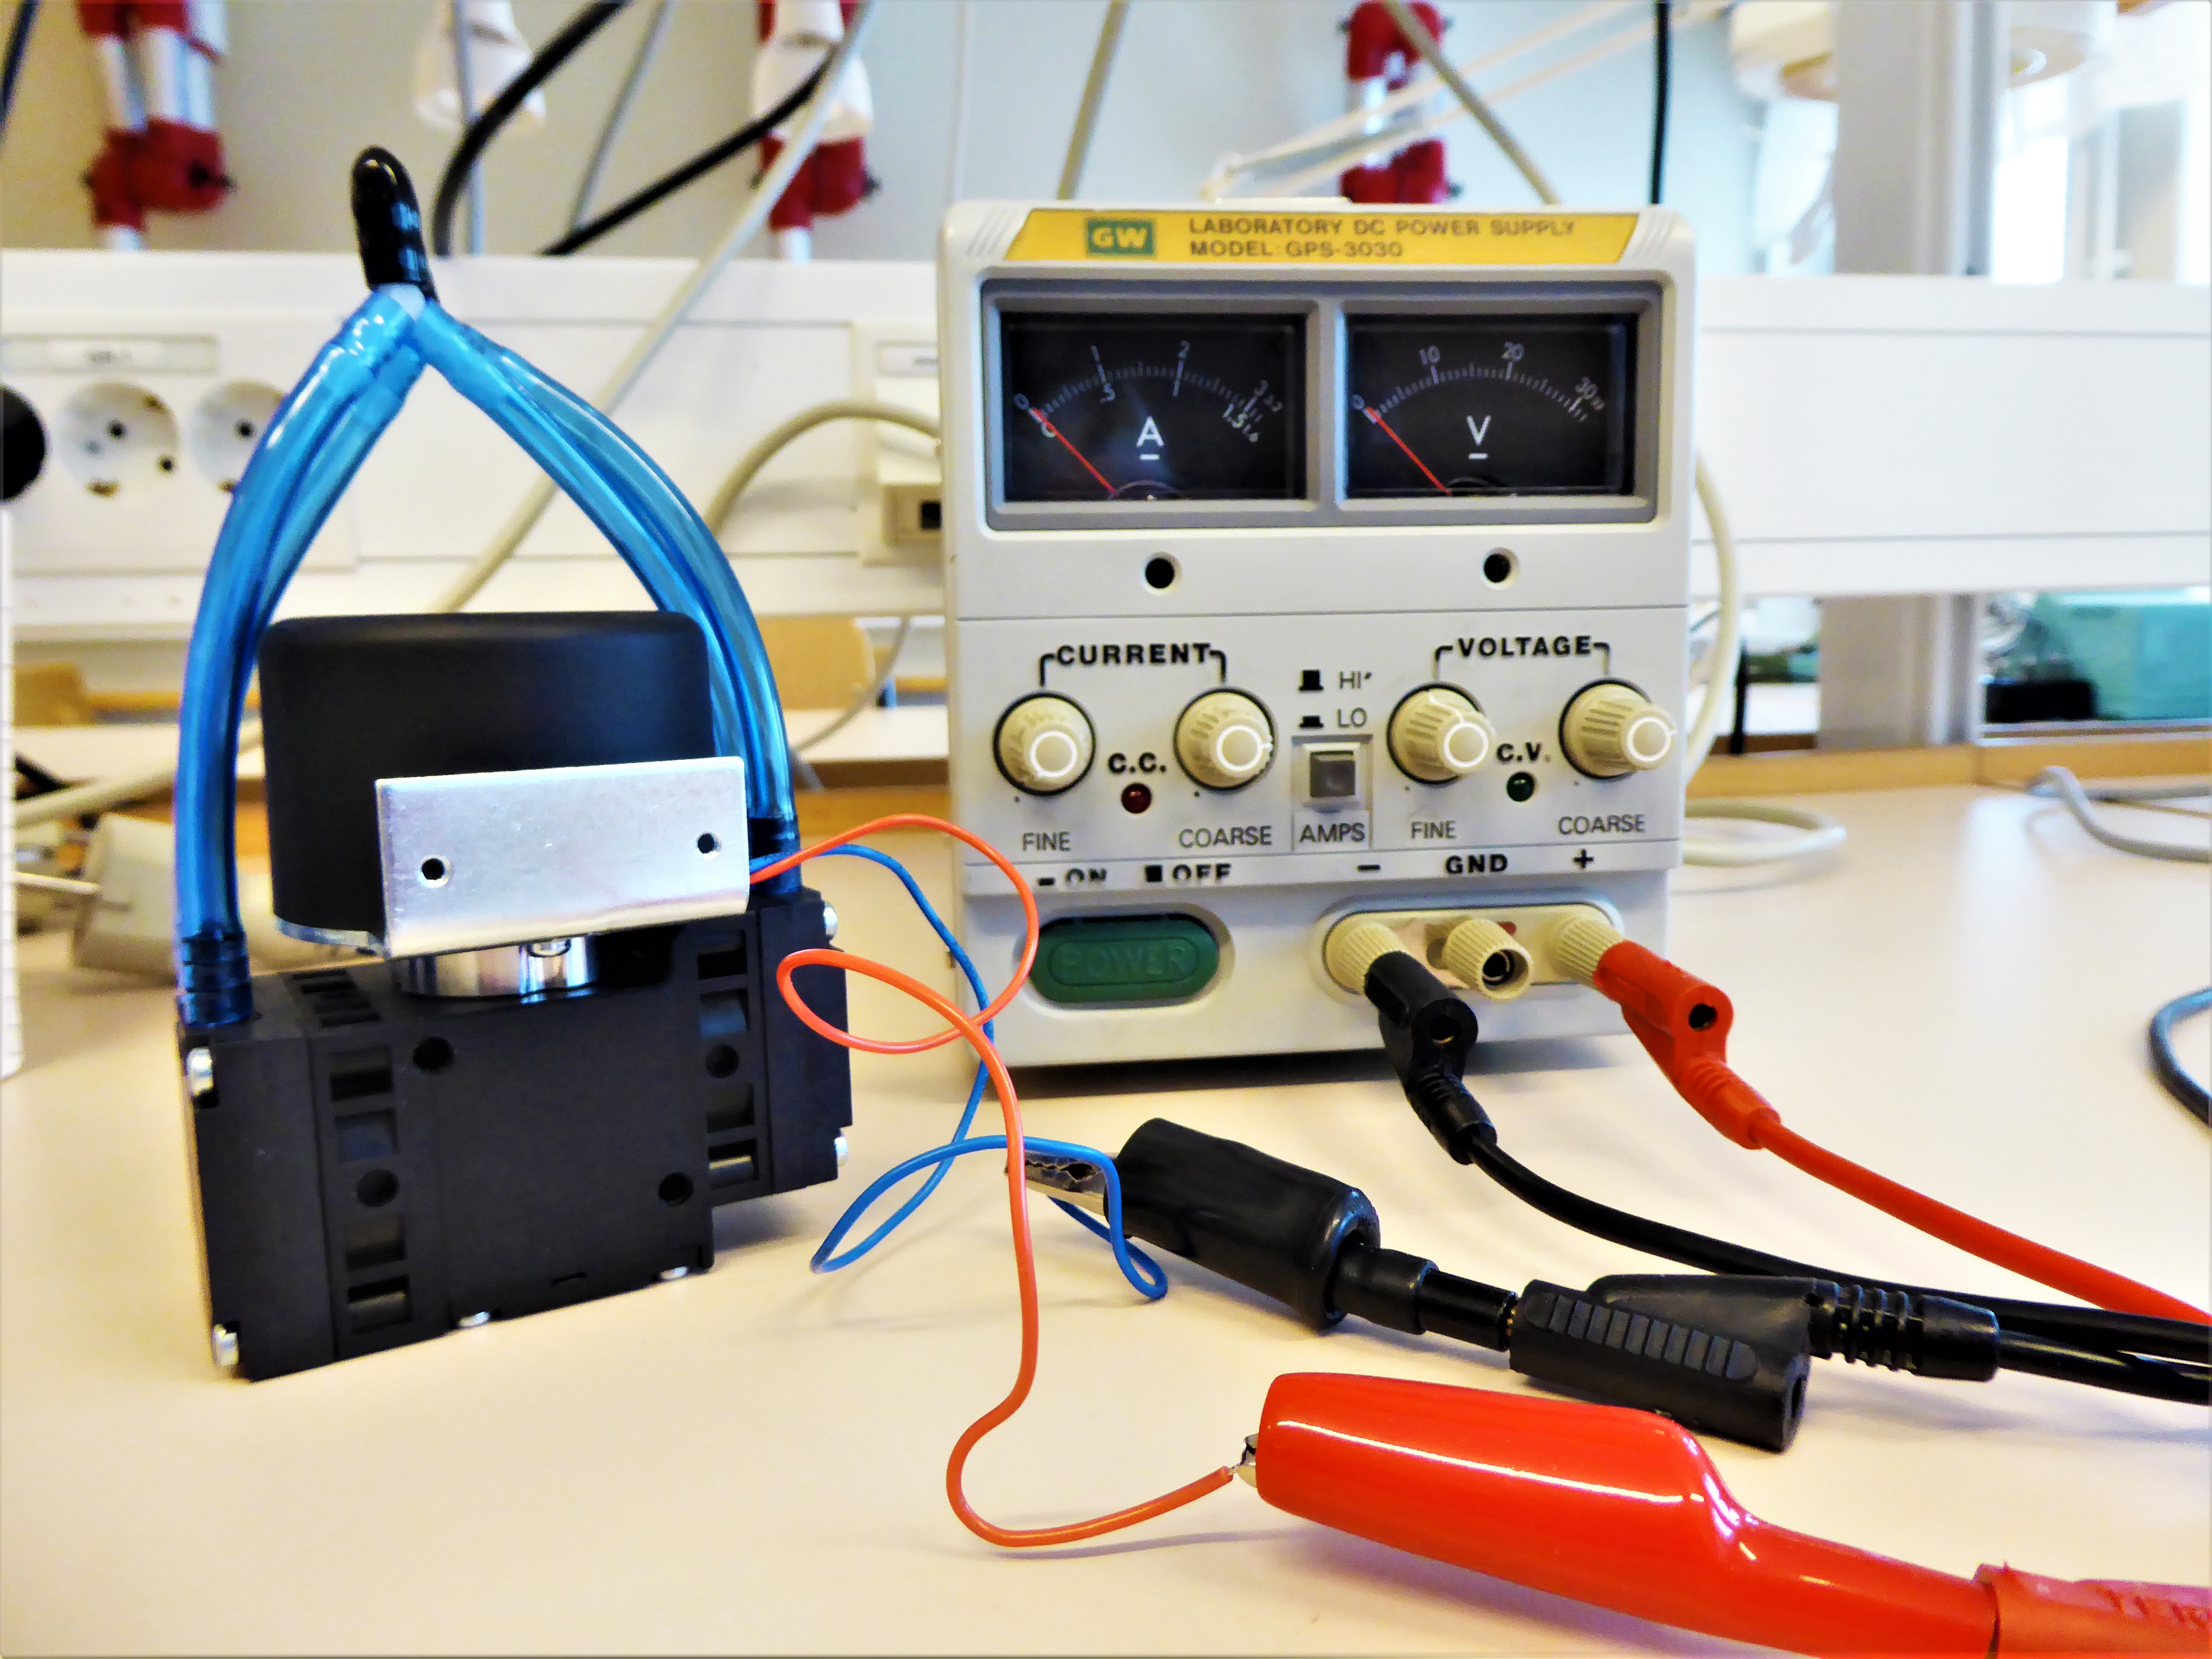
\includegraphics[width=1\linewidth]{5-experiment-verification-and-testing/img/pump-testing.png}
    \end{align*}
    \caption{Photo Showing the Set-up for the Pump Testing in the Laboratory.} \label{fig:pump-testing}
\end{figure}

\subsection{Test 18: Pump Low Pressure}\label{subsection:pumplowpressuretest}

The pump was tested at low pressure using a small vacuum chamber that is capable of going down to \SI{1}{\hecto\pascal}. For this test the chamber was only taken down to \SI{30}{\hecto\pascal} as this is the expected pressure at 24 km, the highest altitude that will be sampled. The experiment set-up can be seen in Figure \ref{fig:pump-low-pressure-set-up}. The pump was connected to the power supply via two cables. It was also screwed into the base plate to prevent it from moving due to its own vibration during the test. A vacuum pump was connected to the chamber wall with a pressure sensor attached to monitor the pressure inside the chamber. 

\begin{figure}[H]
    \begin{align*}
        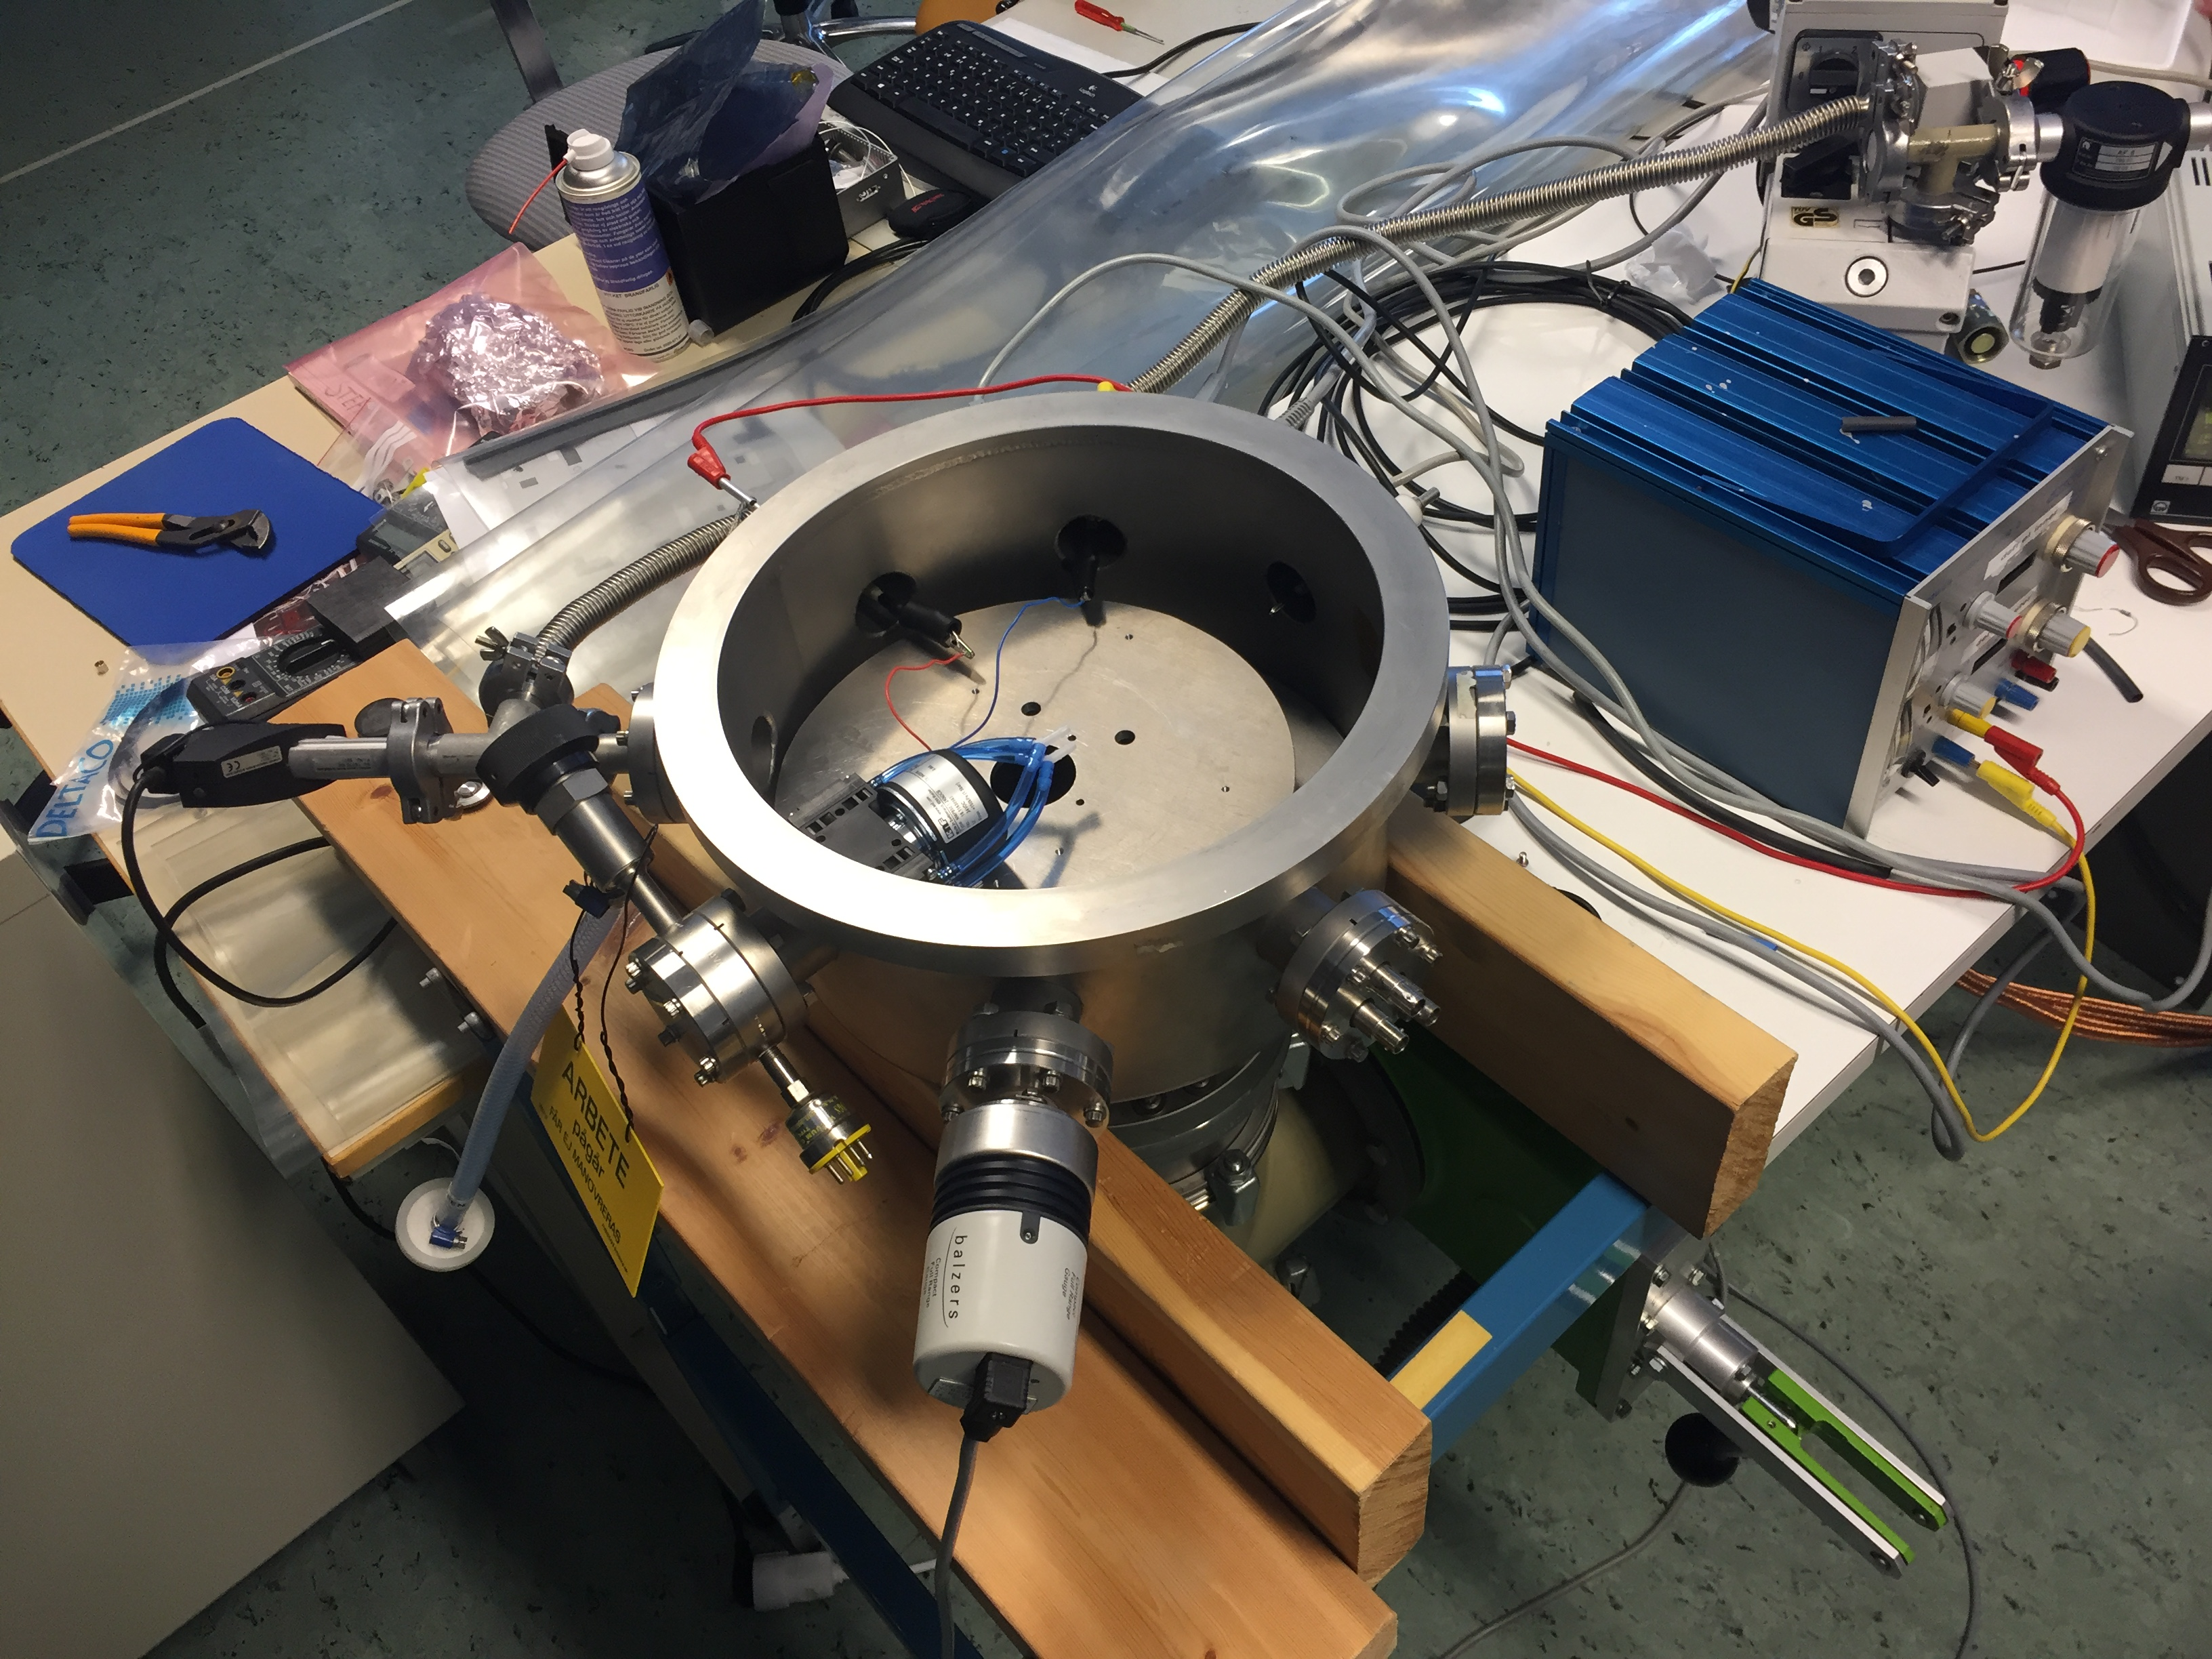
\includegraphics[width=1\linewidth]{5-experiment-verification-and-testing/img/low-pressure-set-up.png}
    \end{align*}
    \caption {Photo Showing the Set-up of the Vacuum Chamber, Power Supply and Vacuum Pump.}\label{fig:pump-low-pressure-set-up}
\end{figure}

The glass top and cage were then placed on top of the sampling bag and pump and the air slowly removed. Figure \ref{fig:pump-low-pressure-progress} shows the test as it was in progress. 

As the air was removed from the chamber a new problem became immediately obvious. Air that was inside the bag before the test was expanding as the pressure decreased until the bag reached around $75\%$ of its total volume. The air had been pushed out of the sampling bag before the test but this had not been completed thoroughly enough. Therefore care must be taken to ensure that there is no, or very very small amounts, of air inside the bag before it enters a low pressure environment. For subsequent tests the pump was used in reverse to suck any remaining air out of the bags. 

\begin{figure}[H]
    \begin{align*}
        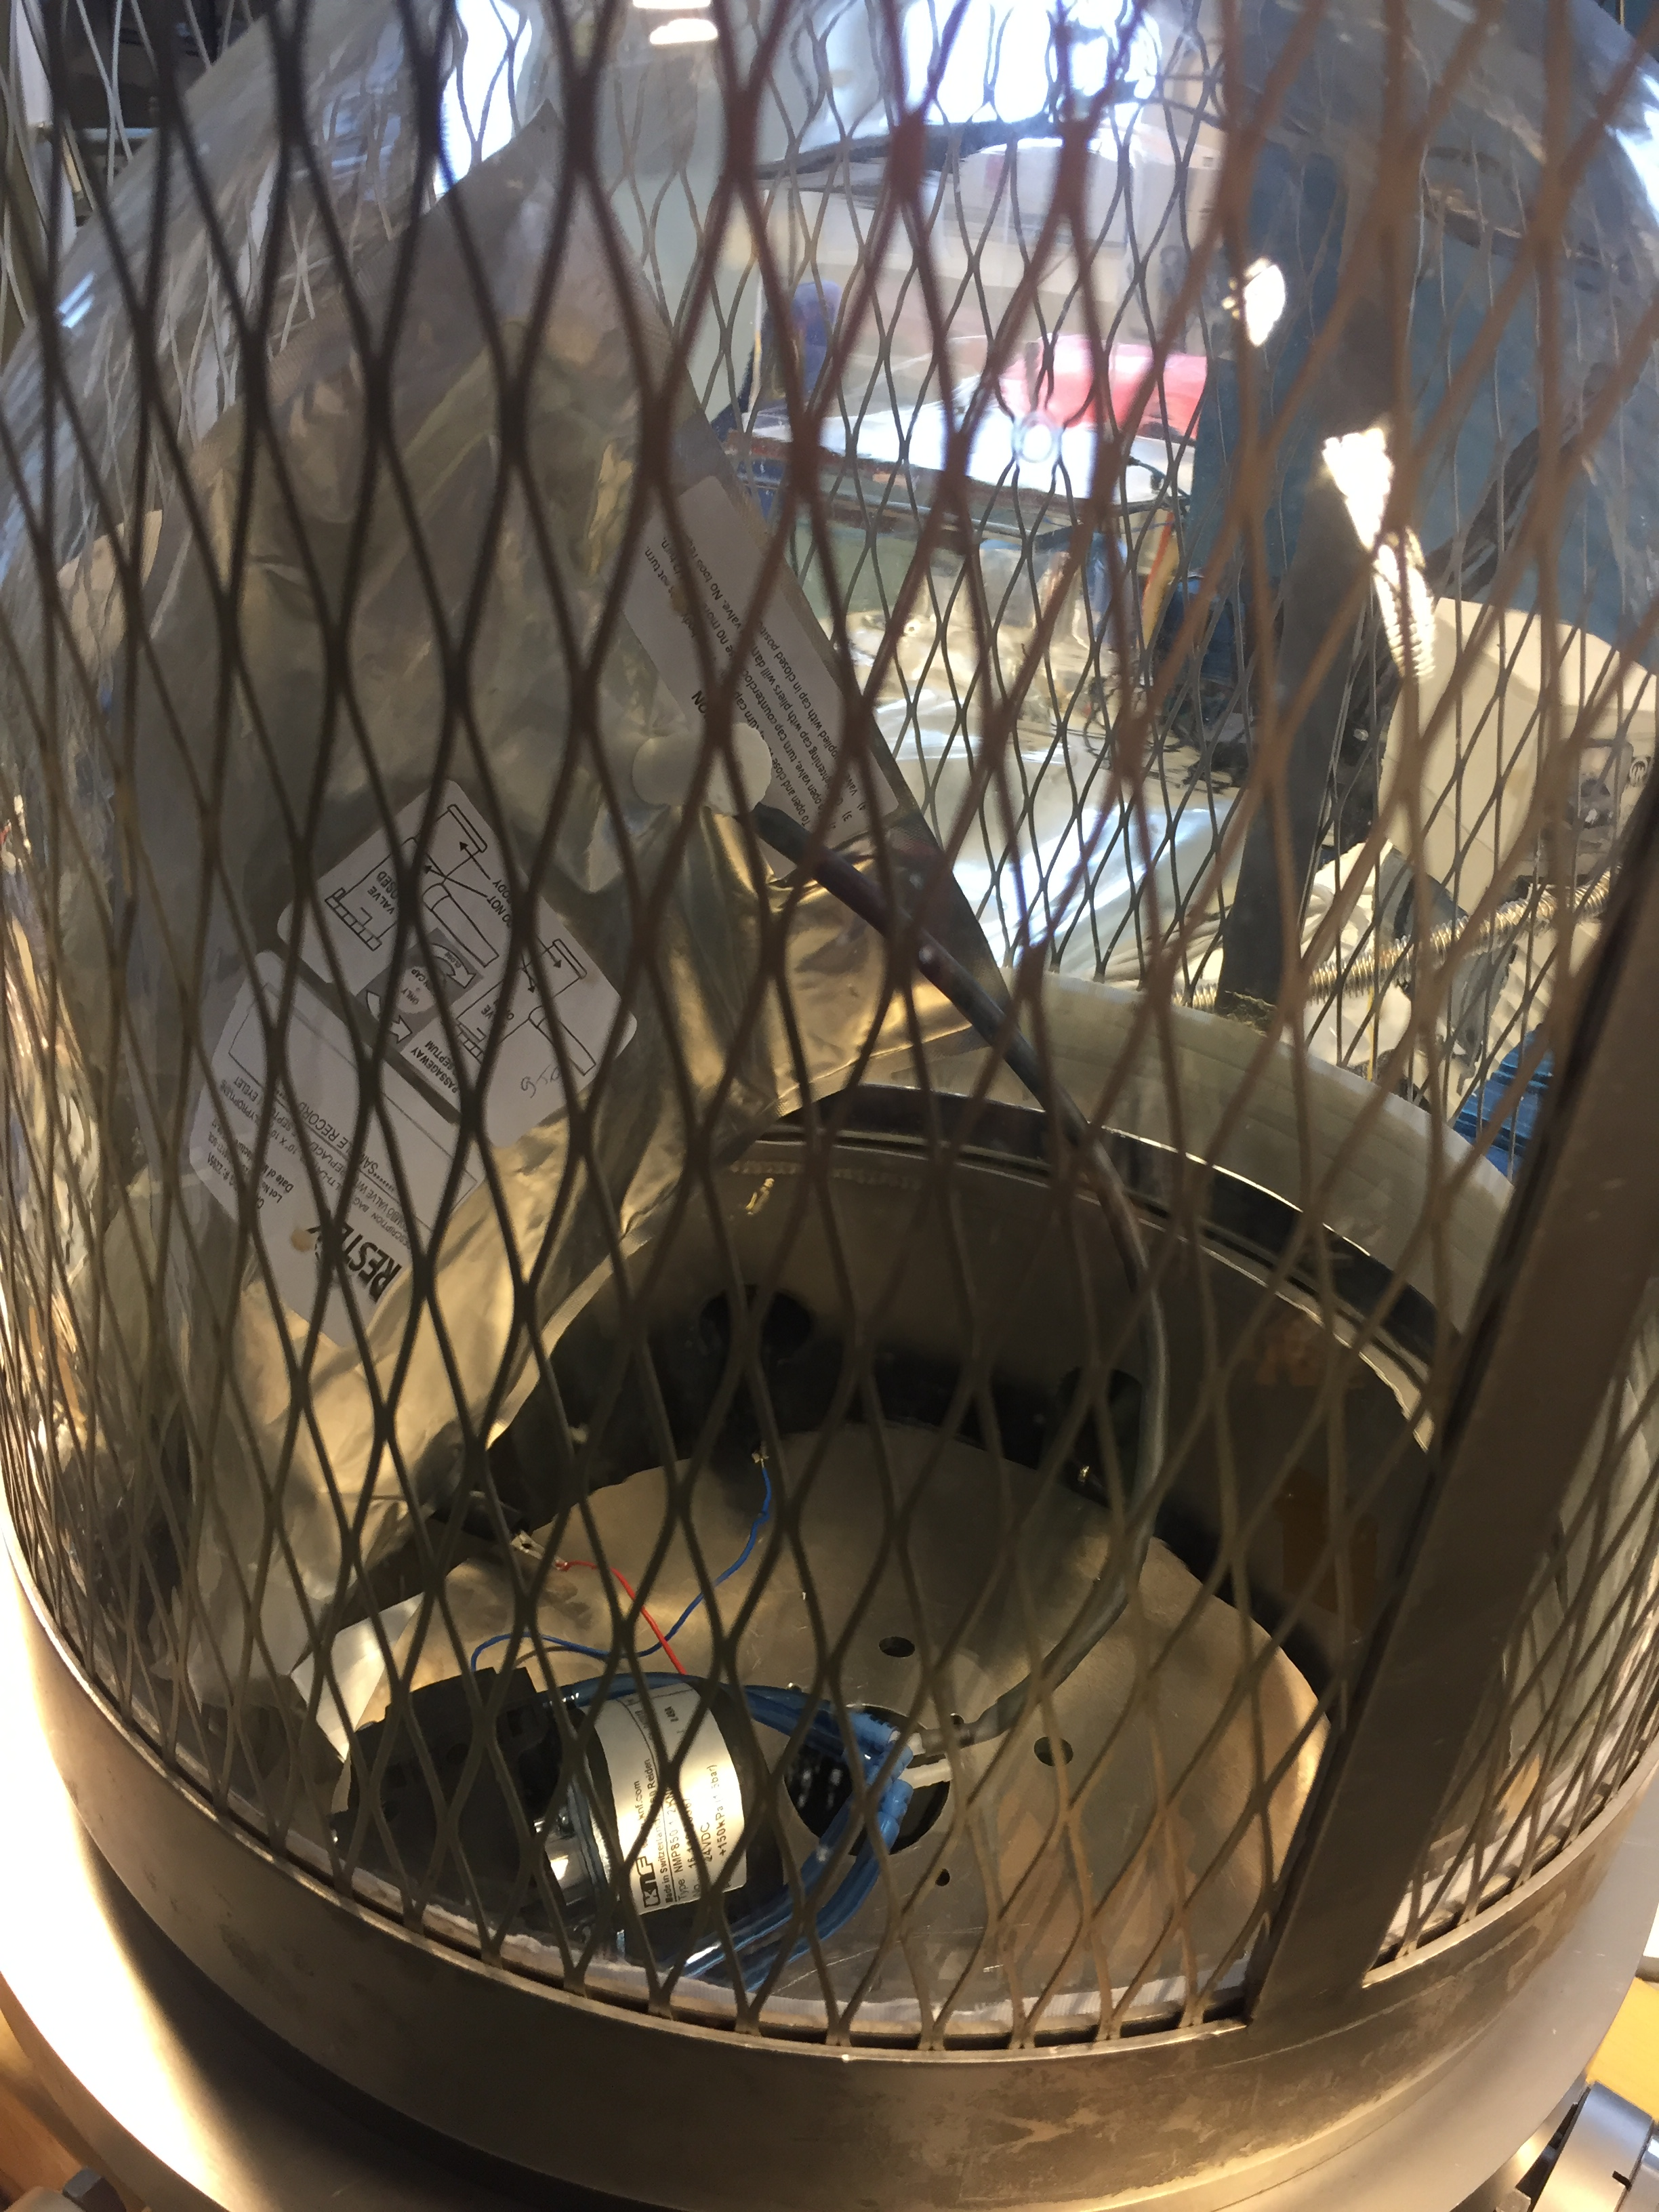
\includegraphics[width=6cm]{5-experiment-verification-and-testing/img/low-pressure-in-progress.png}
    \end{align*}
    \caption {Photo Showing the Pump and Sampling Bag in the Vacuum Chamber During the Test.} \label{fig:pump-low-pressure-progress}
\end{figure}

Repeating the test and using the pump to suck out excess air from the bags the chamber was taken to around \SI{30}{\hecto\pascal}. Once the chamber was at this pressure the pump was switched on and a stopwatch began. Once the bag stopped inflating the stopwatch was stopped. During this test there was also a drop in pressure to \SI{28}{\hecto\pascal} and during a repeat there was a drop to \SI{25}{\hecto\pascal}. This also occurred in later tests. This is not seen as a significant problem as during the flight this is exactly what will happen when testing during ascent. In addition the flow rate increases with increasing outside pressure therefore this is showing our worst case flow rate. It was found that the pump was able to successfully switch on and fill the bag at this altitude with a flow rate of approximately 3 L/min. 

The test was repeated again at \SI{88}{\hecto\pascal}, representing 17 km altitude and \SI{220}{\hecto\pascal}, representing 11 km altitude. Here the flow rates were found to be 3.4 L/min and 4.9 L/min respectively. The results can also be seen in Table \ref{tab:pump-low-pressure-result} and Figure \ref{fig:pump-performance}.

As this test could only provide and approximation due to the lack of equipment such as flow-meters that would have made this test more precise it was later repeated. In the repeat of this test the flow rates were found to be within the same magnitude. The full results can be seen in Section \ref{sec:ExpecterResults} in Table \ref{tab:normal-flow-rates}. 

\begin{table}[H]
\centering

\begin{tabular}{|l|l|l|l|l|l}
\cline{1-5}
Altitude (km) & Pressure Start (hPa) & Pressure End (hPa) & Time (sec) & Flow Rate (LPM) &  \\ \cline{1-5}
24 & 30 & 23 & 60 & 3 &  \\ \cline{1-5}
17 & 87 & 80 & 53 & 3.4 &  \\ \cline{1-5}
11 & 220 & 190 & 37 & 4.9 &  \\ \cline{1-5}
\end{tabular}
\caption{Table showing the time taken until the 3L bag stopped expanding at various different pressures.}
\label{tab:pump-low-pressure-result}
\end{table}

\raggedbottom

\begin{figure}[H]
    \begin{align*}
        \includegraphics[width=11cm]{5-experiment-verification-and-testing/img/pump-performance.jpg}
    \end{align*}
    \caption {Obtained Pump Performance at Low Pressure.} \label{fig:pump-performance}
\end{figure}

\subsubsection{Test 30: Sampling Bag Bursting}
\label{sec:test30result}

A sampling bag was placed in a small vacuum chamber connected to the pump with the same set up as in Test 18, see Figures \ref{fig:pump-low-pressure-set-up} and \ref{fig:pump-low-pressure-progress}. The pump was run for 3 minutes with a full bag to see how the bag reacted. No changes were observed in the bag and no leaks appeared whilst it was in the testing chamber. Upon returning it to atmospheric levels it also appeared to be able to withstand the over pressure. The bag was then left, with the valve closed, on a table where it was handled a little during this time. Approximately 30 minutes after the test the bag made an audible popping noise and air leaked out. The damage that occurred to the bag during the burst can be seen in Figure \ref{fig:bag-burst-front} for the front of the bag and Figure \ref{fig:bag-burst-back} for the back of the bag.

\begin{figure}[H]
    \begin{align*}
        \includegraphics[width=0.7\linewidth]{5-experiment-verification-and-testing/img/bag-burst-front_rescaled.png}
    \end{align*}
    \caption {Photo Showing the Extent of Damage on the Front of the Bag Due to Bursting.} \label{fig:bag-burst-front}
\end{figure}

\begin{figure}[H]
    \begin{align*}
        \includegraphics{5-experiment-verification-and-testing/img/bag-burst-back_rescaled.png}
    \end{align*}
    \caption {Photo Showing the Extent of Damage on the Back of the Bag Due to Bursting.} \label{fig:bag-burst-back}
\end{figure}

This kind of bag failure could occur if bags are overfilled, particularly during ascent.

Next the system was set-up in the same way with a new bag. This time the pump was continuously run until failure occurred. This took around 6 minutes. The bag failed along the lower seam close to the valve and also at the valve connection. At the valve connection the bag ripped just above the valve. This time the burst was more energetic with the bottom of the bag moving outwards. Upon inspection the bottom of the bag was completely open and the part of the bag connected to the valve partially ripped open. In addition at the top of the bag small failures similar to those seen in Figure \ref{fig:bag-burst-front} were seen again. It is therefore thought that the bag was starting to fail at both the top and the bottom of the bag and but the bottom failed first.

The damage can be seen in Figures \ref{fig:seam-break} and \ref{fig:valve-rip}. It should be noted that the white bag valve was pulled off after the test and before photos were taken.

\begin{figure}[H]
    \begin{align*}
        \includegraphics[width=0.45\linewidth]{5-experiment-verification-and-testing/img/bag-seam-break.jpg}
    \end{align*}
    \caption {Photo Showing the Damage Sustained to the Bottom of the Bag After Bursting Due to Continuous Pumping.} \label{fig:seam-break}
\end{figure}

\begin{figure}[H]
    \begin{align*}
        \includegraphics{5-experiment-verification-and-testing/img/bag-valve-break_rescaled.png}
    \end{align*}
    \caption {Photo Showing Where the Bag Ripped Around the Valve.} \label{fig:valve-rip}
\end{figure}

This kind of bag failure could occur if there is a software error that results in the pump not switching off or a valve not closing, or if there is a malfunction in one of the valves which means it fails to close.

From the damage seen on the bags and from witnessing the burst it can be concluded that, as long as the bags are well secured to the valves at the bottom and through the metal ring at the top, bag bursting during flight would not cause damage to any other components on board. Even during the more energetic burst that occurs from continuous pumping the bag remained fixed to the valve connection and experienced no fragmentation. The consequences of a single bag burst would be limited to loss of data and a disturbance to audio frequencies. 

\subsection{Test 29: Pump Current under Low Pressure}
\label{sec:test29result}

This test was set up in the same way as above in Test 18, see Figure \ref{fig:pump-low-pressure-set-up} and \ref{fig:pump-low-pressure-progress}. The addition to this test was a multimeter to read the current that the pump was drawing. The pump was tested once with the outlet attached to a bag and once with the outlet sealed. This provides the current when the pump is pumping into an ambient pressure and into a higher pressure.

In general it was found for both cases that decreasing the pressure, or increasing the altitude, lead to a decrease in pump current draw. It was noted that there was an increase in current draw in between sea level conditions and 11 km altitude conditions. However as the lowest sampling point it intended to be at 11 km this should not be a problem for the experiment. The full results can be seen in Table \ref{tab:pumpcurrentpressure}. 

\begin{table}[H]
\centering

\begin{tabular}{|l|l|l|l|}
\hline
Altitude (km) & Pressure (hPa) & Into Bag Current (mA) & Into Seal Current (mA) \\ \hline
20 & 57 & 140 & 138 \\ \hline
18 & 68 & 150 & 141 \\ \hline
16 & 100 & 161 & 146 \\ \hline
12 & 190 & 185 & 175 \\ \hline
9 & 300 & - & 200 \\ \hline
6 & 500 & - & 242 \\ \hline
0 & 1013 & - & 218 \\ \hline
\end{tabular}
\caption{Table showing how the current draw of the pump changed with outside air pressure for two different conditions. The first pumping into a sampling bag and the second pumping into a sealed tube.}
\label{tab:pumpcurrentpressure}
\end{table}

A graphical representation of these results are shown in Figures \ref{fig:pumpcurpresbag} and \ref{fig:pumpcurpres}. From the table and figures it can be seen that the current draw is higher during the bag filling than during the sealed case. As the experiment will sample between 11 km and 24 km it can be concluded that the highest current draw will occur during the 11 km altitude sample and can be expected to be around 200 mA. 

\begin{figure}[H]
    \begin{align*}
        \includegraphics[width=1\linewidth]{5-experiment-verification-and-testing/img/pump-cureent-pressure.png}
    \end{align*}
    \caption {Graph Showing the Expected Current Values When the Pump is Pumping Air Into a Bag Based Upon the Results Obtained.} \label{fig:pumpcurpresbag}
\end{figure}


\begin{figure}[H]
    \begin{align*}
        \includegraphics[width=1\linewidth]{5-experiment-verification-and-testing/img/pump-current-pressure.png}
    \end{align*}
    \caption {Graph Showing the Expected Current Values When the Pump is Pumping Air Into a Sealed Outlet Based Upon the Results Obtained and the Data Shown In Figure \ref{fig:pumpflowcur}.} \label{fig:pumpcurpres}
\end{figure}

By looking at the data from both Test 18 and Test 29 a relationship can be seen between the outside air pressure, the flow rate of the pump and the current draw of the pump. 

\subsection{Test 17: Sampling bags' holding times and samples' condensation verification}
\label{sec:test17result}

The main objective of this test was to flush eight 1 L sampling bags with nitrogen, the same way it will be done for the flight. After the flushing is done, fill them with a dry gas and leave them outside for 6, 14, 24 and 48 hours. Then analyze two sampling bags after each time duration and see if the concentration of gases inside has changed. 

A dry gas is a gas of high concentration of $CO$ and low $H_2O$ and its exact concentration can be known by comparison to the calibrating gas in the Picarro analyzer. Therefore, the concentration when sampling the bags is known and it can be compared with the concentration after analysis. If the sampling bags can hold the samples for 48 hours then when analyzing, the concentration of gases should not change. If condensation occurs that will be seen as an increase in water vapour concentration. 

Note that the size of the sampling bags was not the same as the size that will be used during the experiment. The reasons were availability of 1 L sampling bags at FMI and a first assumption that the size would not affect the results. The sampling bags were exactly the same model/material.


This test was realized at FMI in Sodankyl\"{a}. Eight Multi-Layer Foil bags of 1 L volume were connected to SMC valves as shown in Figure \ref{fig:bag-valve-quick-connector} and all together connected in series with stainless steel tubes as can be seen in Figure \ref{fig:bags-test-set-up}.

\begin{figure}[H]
    \begin{align*}
        \includegraphics[width=1\linewidth]{5-experiment-verification-and-testing/img/bag-valve-quick-connector.jpg}
    \end{align*}
    \caption {1 L Sampling Bag With SMC Valve Attached to It. The Valve is at One of the Ends of the System so a Quick Connector is Connecting it to the Tube That Goes to the Nitrogen Bottle/Vacuum Pump.} \label{fig:bag-valve-quick-connector}
\end{figure}


\begin{figure}[H]
    \begin{align*}
        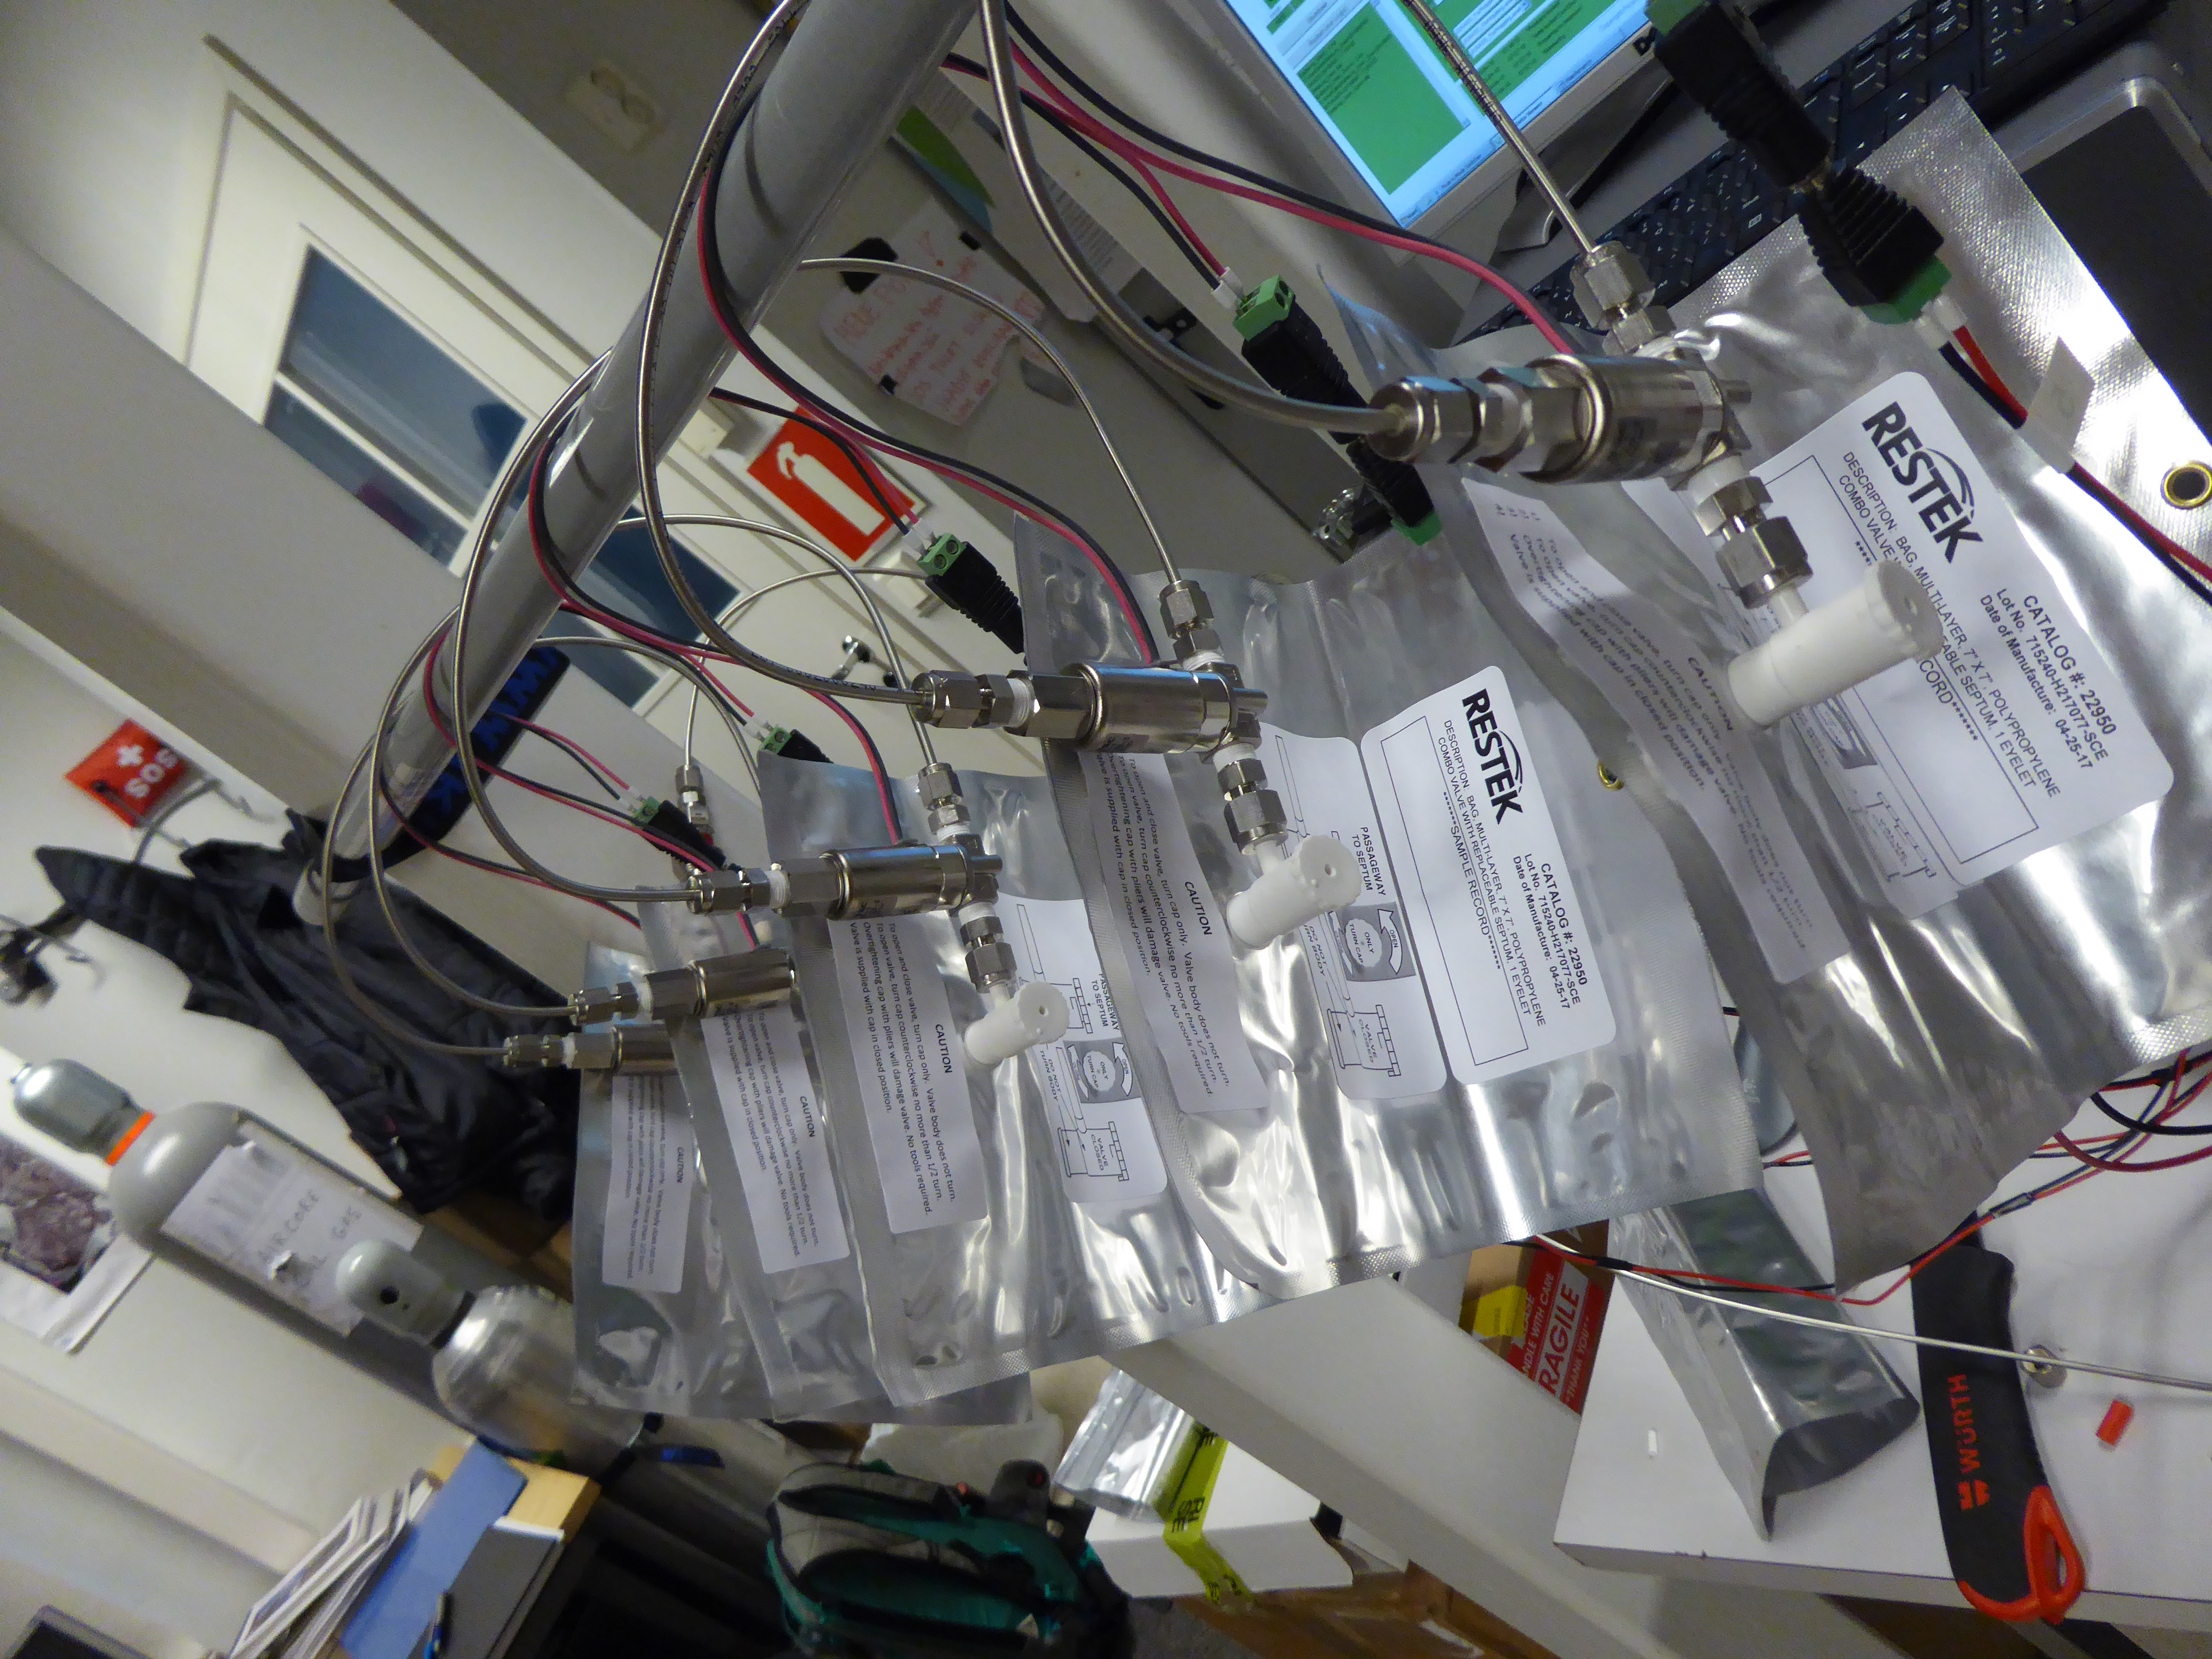
\includegraphics[width=1\linewidth]{5-experiment-verification-and-testing/img/bags-test-set-up.jpg}
    \end{align*}
    \caption {Sampling Bags System Connected in Series.} \label{fig:bags-test-set-up}
\end{figure}

Figure \ref{fig:bags-test-general-overview} shows a general overview of the experiment set up before the sampling bags were attached to the SMC valves. The picture shows the eight SMC valves hanging on a bar and red and black cables connecting them to the switches. It can also be seen a nitrogen bottle standing at the right side of the table and a vacuum pump under the table. Figure \ref{fig:nitrogen-vacuum-valve} shows the pressure sensor on the table, a flow-metre, a needle valve that adjusts the flow rate and a valve. This valve was used to control the filling and flushing of the sampling bags realized with nitrogen. The position shown in Figure \ref{fig:nitrogen-vacuum-valve} is for vacuuming, the pump is sucking the air from the sampling bags and the nitrogen tube is closed. The valve position for filling is the opposite, opening the nitrogen tube and closing the vacuum. There is also an intermediate position that closes both, nitrogen and vacuum. 



\begin{figure}[H]
    \begin{align*}
        \includegraphics[width=1\linewidth]{5-experiment-verification-and-testing/img/bags-test-general-overview.jpg}
    \end{align*}
    \caption {General Overview of the test Set up Before the Sampling Bags Were Attached to the Valves} \label{fig:bags-test-general-overview}
\end{figure}



\begin{figure}[H]
    \begin{align*}
        \includegraphics[width=1\linewidth]{5-experiment-verification-and-testing/img/nitrogen-vacuum-valve.jpg}
    \end{align*}
    \caption {Valve that Controls Filling/Vacuum in of the Sampling Bags. Pressure Sensor, Flow-metre and Needle Valve.} \label{fig:nitrogen-vacuum-valve}
\end{figure}


The procedure during the test was as follows: 
\begin{itemize}
    \item Set up all the connections between pump, nitrogen bottle, valves system in series. 
    \item Attach the sampling bags to the SMC valves. 
    \item Start flushing the tubes with nitrogen. For this all the sampling bags' valves are closed. 
    \item Adjust the flow rate of nitrogen at 500 ml/min. 
    \item Open sampling bags' manual valves (not to be confused with the SMC valves which are still all closed).
    \item Turn on valve 1. Fill sampling bag number 1 for 2 minutes. Turn off valve 1. Repeat it for the seven sampling bags left.  
    \item Change the valve seen in Figure \ref{fig:nitrogen-vacuum-valve} to vacuum position and empty the bags.
    \item Flush the tubes after all the sampling bags have been emptied. This is to remove as much air as possible that could be left inside the sampling bags.
    \item Repeat the flushing for two more times. 
    \item Change the nitrogen bottle for the dry gas bottle. 
    \item Flush the tubes with nitrogen. 
    \item Fill the eight sampling bags one by one. 
    \item Take the sampling bags outside as shown in Figure \ref{fig:bags-outside} to simulate the conditions at which they will be exposed after landing. 
\end{itemize}

\begin{figure}[H]
    \begin{align*}
        \includegraphics[width=0.75\linewidth]{5-experiment-verification-and-testing/img/bags-outside_rescaled.png}
    \end{align*}
    \caption {Sampling Bags Left Outside Waiting to be Analyzed.} \label{fig:bags-outside}
\end{figure}

After each of the mentioned times, 6, 14, 24 and 48 hours, two sampling bags were taken inside the laboratory to be analyzed. The procedure to analyze was: 
\begin{itemize}
    \item Have the dry gas flowing through the Picarro analyzer for at least one hour before the analysis. This is to avoid having moisture inside the tubes and have stable measurements of concentrations.
    \item Flush the tubes in between the two sampling bags with dry gas. For that the dry gas has to be disconnected from the analyzer and moisture would get into the Picarro. To avoid this, calibrating gas is flowing through the analyzer while the tubes are being flushed.
    \item Connect the system formed by two sampling bags with one end to the dry gas bottle and the other to the Picarro inlet.
    \item Wait for one hour until the readings of dry gas concentrations are stable. 
    \item Open the valve of the first sampling bag. 
    \item Right after the first sampling bag is empty, close its valve and open the valve for the next one. 
    \item Keep the dry gas flowing for one more hour after analysis. 
\end{itemize}

After analyzing the sampling bags the obtained results are presented in Figure \ref{fig:test17-results}.

\begin{figure}[H]
    \begin{align*}
        \includegraphics[width=1\linewidth]{5-experiment-verification-and-testing/img/test17-results.jpg}
    \end{align*}
    \caption {Obtained Variation in Concentration for (a) $CO_2$ in ppm, (b) $CO$ in ppb, (c) $CH_4$ in ppb and (d) $H_2O$ in ppb.} \label{fig:test17-results}
\end{figure}


It should be mentioned that the results were not at all what was expected. If the sampling bags held the gases for 48 hours, the analyzed concentration should have been the same as the dry gas used to fill them or the variation should have been smaller. 

A possible explanation for this results could be that the emptying of the sampling bags was not done rigorously enough and that some air/nitrogen was left inside which diluted in the dry gas and changed the concentrations. This effect is even increased due to the smaller size of the used sampling bags (1 L instead of 3 L). This would also explain why the results don't follow any pattern. 

The general outcome of this test was that the team realized that the flushing of the sampling bags is a very delicate process. This test was also useful to decide that the flushing of the sampling bags should be done with dry gas instead of nitrogen in order to minimize the effects of the nitrogen diluting in the samples. 

This test had to and was repeated, using the set-up described in Section 4, with some differences. This time 3L bags were flushed with dry gas and left outside for 15, 24, 48 hours. After the flushing was done, two bags for each time were filled with 0.5 L and 1L of dry gas and left outside. Then they were analyzed and checked if the sample concentrations were the same or close enough with the reference values of the filled dry gas.

The obtained results are shown in Figure \ref{fig:test17-resultsSEP}. The blue points represent the sampling bags with the 0.5L sample, while the red points show the sampling bags with the 1L sample. Sampling Bag No1 with the sampling bag No4 were analyzed after 15 hours. The pair of sampling bags No2 and No5 were analyzed after 24 hours and the last pair of sampling bags, No4 and No6 after 48 hours.  

\begin{figure}[H]
    \begin{align*}
        \includegraphics[width=1\linewidth]{5-experiment-verification-and-testing/img/test17resultsSEP.jpg}
    \end{align*}
    \caption {Obtained Variation in Concentration for (a) $CO_2$ in ppm, (b) $CO$ in ppb, (c) $CH_4$ in ppb and (d) $H_2O$ in $\%$.} \label{fig:test17-resultsSEP}
\end{figure}

The results were very good in general with the $CO_2$ concentration differences not higher than 2 ppm. The bags with the 0.5L sample gave bigger $CO_2$ concentration differences and higher humidity for all the tested times. For the bags that analyzed after 48 hours, the humidity was two times higher for the 0.5L sample compared to the 1L sample. If water goes through the walls of the bags at the same rate for both bags then it is normal that sampling bags with larger amounts of sampled air have lower humidity concentrations. Therefore, for better results, the air left in the sampling bags at sea level pressure must be the maximum possible.


% Flushing with nitrogen may alter the results. 

\subsubsection{Test 4: Low Pressure}
\label{sec:test4results}
\textbf{Styrofoam}

The same vacuum chamber was used as in Tests 18 and 29. The Styrofoam was measured on each side before it was placed in the chamber. It was then taken down to 5 hPa and held there for 75 minutes. It was then removed and the sides were measured again. It was found that there was no significant change in dimensions. The results can be seen in Table \ref{tab:styrofoam-test-result}.

\begin{table}[H]
\centering
\begin{tabular}{|l|l|l|}
\hline
Side & Before (cm) & After (cm) \\ \hline
A & 9.610 & 9.580 \\ \hline
B & 9.555 & 9.550 \\ \hline
C & 9.560 & 9.565 \\ \hline
D & 9.615 & 9.610 \\ \hline
E & 9.615 & 9.615 \\ \hline
F & 9.555 & 9.550 \\ \hline
G & 9.605 & 9.605 \\ \hline
H & 5.020 & 5.020 \\ \hline
I & 5.025 & 5.025 \\ \hline
J & 5.015 & 5.015 \\ \hline
K & 5.020 & 5.025 \\ \hline
\end{tabular}
\caption{Styrofoam Size Before and After Vacuum.}
\label{tab:styrofoam-test-result}
\end{table}
%\begin{table}[H]
\begin{tabular}{|l|l|l|}
\hline
Side & Before (cm) & After (cm) \\ \hline
A & 9.610 & 9.580 \\ \hline
B & 9.555 & 9.550 \\ \hline
C & 9.560 & 9.565 \\ \hline
D & 9.615 & 9.610 \\ \hline
E & 9.615 & 9.615 \\ \hline
F & 9.555 & 9.550 \\ \hline
G & 9.605 & 9.605 \\ \hline
H & 5.020 & 5.020 \\ \hline
I & 5.025 & 5.025 \\ \hline
J & 5.015 & 5.015 \\ \hline
K & 5.020 & 5.025 \\ \hline
\end{tabular}
\caption{Styrofoam Size Before and After Vacuum.}
\label{tab:styrofoam-test-result}
\end{table}

As some sides are measured slightly bigger after and some slightly smaller it is thought this is due to the measuring technique and not due to changes in the Styrofoam. It is thought the result from side A could be due to deforming the Styrofoam with calipers or a misread original length.

\begin{figure}[H]
    \begin{align*}
        \includegraphics[width=0.4\linewidth]{appendix/img/test-results/styrofoam-round-two.jpg}
    \end{align*}
    \caption {Picture Showing how the Styrofoam was Labeled for the Test.} \label{fig:styrofoam-test-labeling}
\end{figure}

\textbf{Airflow}

After the first airflow in vacuum test failed due to datalogging errors the airflow test was repeated. In this repeated test all of the Brain was placed into the vacuum chamber and one bag attached. It was not possible to attach more than one bag due to space restrictions. A view inside the vacuum chamber can be seen in Figure \ref{fig:insidevacuum}.


\begin{figure}[H]
    \begin{align*}
        \includegraphics[width=0.67\linewidth]{appendix/img/test-results/vacuum-test/inside-chamber-square.jpg}
    \end{align*}
    \caption {Picture Showing inside of the Vacuum Chamber During the Test.} \label{fig:insidevacuum}
\end{figure}

To confirm the airflow rates the vacuum chamber was then taken down to from 400 hPa to 5 hPa in steps and the airflow rate logged. The results can be seen in Figure \ref{fig:airflowvacuum}.


\begin{figure}[H]
    \begin{align*}
        \includegraphics[width=1\linewidth]{appendix/img/test-results/vacuum-test/airflowvacuumtestgraph.jpg}
    \end{align*}
    \caption {Graph Showing how the Airflow Rate is Changing with Ambient Pressure.} \label{fig:airflowvacuum}
\end{figure}

Sampling will take place between 200 hPa and 22 hPa, this area is seen in greater detail in Figure \ref{fig:airflowvacuumregion}. From this graph it can be seen that the airflow rate is varying from 1.2 LPM to 0.1 LPM.


\begin{figure}[H]
    \begin{align*}
        \includegraphics[width=1\linewidth]{appendix/img/test-results/vacuum-test/airflow-vacuum-graph-sampling-area.jpg}
    \end{align*}
    \caption {Graph Showing how the Airflow Rate is Changing with Ambient Pressure in the Sampling Region.} \label{fig:airflowvacuumregion}
\end{figure}


It was noted that the airflow rate seemed to be very low when compared to the rate at which the bag was inflating. For example for the first sampling point the flow rate was around 0.4 LPM and was filled for 44 seconds. This would imply that the bag was 10\% full with 0.3 L, however from visual inspection it was clear the bag was at least 75\% full. When the bag was brought back to sea level pressure the amount of remaining air in the bag was inspected. It appeared there was approximately 0.3 L left in the bag, as seen in Figure \ref{fig:remainingair}. This led to the conclusion that the airflow rate displayed is the equivalent airflow at sea level.  

\begin{figure}[H]
    \begin{align*}
        \includegraphics{appendix/img/test-results/vacuum-test/remaining-air-table_rescaled.png}
    \end{align*}
    \caption {Picture Showing the Air Remaining in the Bag After Returning to Sea Level Pressure.} \label{fig:remainingair}
\end{figure}


\textbf{Software}

With the same set-up as the airflow low pressure testing the software was tested to verify if it was operating as intended and that the conditions for stopping sampling were working.

First the software was run as it will be during flight. As the pressure inside the chamber was dropped it was possible to see through the LEDs on board the PCB the system going through the flight actions. When the first sampling altitude was reached the lights came on for the flushing valve and pump indicating the system was flushing. After one minute these lights went out and the first valve opened. For the first sampling point it was possible to see the bag inflate providing extra visual confirmation that the system is operating as intended. 

The next check was to see if our conditions for stopping sampling were working. Testing with the initial sampling schedule meant that the time  stopper always occurred first and worked well. The pressure threshold stopper also worked well with the system stopping sampling if the defined pressure range was left. Our third stopper is based on pressure and compares the pressure inside the bag to the ambient pressure to ensure we do not overpressure the bags. Interestingly it was found that this pressure was not being reached even after filling the bags continuously for three minutes, three times our time limit. 

This shows that the maximum allowed pressure for the bags is not the pressure when the bag is 3L full but when the air in the bag has been compressed. This reduces the risk of bags bursting significantly.


\textbf{Temperatures}

As it is not possible to complete a thermal vacuum test in addition to the thermal testing  temperatures were also monitored inside the vacuum chamber. Particular attention was paid to the CAC valve which will be on for the entire flight. From Figure \ref{fig:CACvalvetemp} it can be seen that after 2 hours the temperature is leveling off at around 68$\degree{C}$. This is still well within the operating temperature range of the valve. In addition this was also held at 5 hPa which is a lower pressure than the minimum expected. However this is close to the melting point of the Styrofoam which is at 75$\degree{C}$ so care must be taken to ensure there is no contact between the valve and Styrofoam. In the actual flight the valve is expected to be cooler than this due to the ambient temperature being lower.


\begin{figure}[H]
    \begin{align*}
        \includegraphics[width=0.8\linewidth]{appendix/img/test-results/vacuum-test/valve-temperature.jpg}
    \end{align*}
    \caption {Graph Showing how the Temperature of the CAC Flushing Valve Changes over Time at 5 hPa.} \label{fig:CACvalvetemp}
\end{figure}

The temperature of the pressure sensor, PCB, Pump and Manifold was also monitored with continuous use. After one hour and 48 minutes during the same test as the valve temperature the pressure sensor was found to reach 39$\degree{C}$. After one hour and 24 minutes during the flow rate monitoring test where the sensors, pump, and one manifold valve were on continuously the PCB temperature sensor was at 43$\degree{C}$, the pump at 42$\degree{C}$ and the manifold at 33$\degree{C}$. As the pump will never be on for more than a few minutes at a time there is not any concern that this temperature will ever be reached during flight.

\subsubsection{Test 24: Software and Electronics Integration}
The different type of sensors were integrated one at time with the Arduino. The airflow sensor was first sensor to be integrated. The only problem with this sensor was the lack of calibration to give the correct data. Whilst at FMI this sensor was calibrated using another airflow sensor at FMI. The next sensor to be integrated was the temperature sensor. After several failed attempts to establish a connection to the sensor, a library, based on the information from the sensors datasheet was made. With this library communication was successfully established. During testing some problems were discovered with the temperature sensors as they stopped giving data back when exposed to colder temperatures. This was fixed by implementing a new piece of software code. Before the integration of the pressure sensor it had been expected the need of a self made library, despite this several changes was needed to the library to make the sensor responsive. \par
It was discovered that the pressure sensor on board the PCB wouldn't function while the other pressure sensors when connected to the SPI bus. Parasitic capacitance was suggested to be the culprit when looking on the SPI bus with an oscilloscope. During an telephone conference with our mentors another more reasonable theory was put forwards. Since the SPI was designed to function for short distances only the long cables connecting the outside pressure sensors caused reflections in the bus. The solution was to disregard the pressure sensor on the PCB since it was not a critical sensor.\par
When all the sensors had been integrated the sensors where tested together. The result was all the sensors, exept the PCB pressure sensor, working without interfering with each other.

\subsubsection{Test 5: Thermal Test}\label{thermaltestresults}
The thermal chamber used was the one at FMI. It could go down to between $-40\degree{C}$ and $-90\degree{C}$. A few long run tests were done slowly going down to a temperature and stabilizing before lowering the temperature again to safely test that everything worked when it was below $-20\degree{C}$ outside and if it would handle a 4h $-40\degree{C}$ test. The long run test for $-40\degree{C}$ still needs to be done, because the temperature sensors gave an error and stopped showing data meaning the test was interrupted. With no temperature data the heaters could not be operated properly and the risk for damage was high enough to stop the testing to make sure no components were harmed.

To start with, only the AAC was put into the freezer. In the following Figures the vertical dotted line indicates where the sensor started to throw the error.
The first test slowly went down to $-20\degree{C}$ before it stabilized, then it went down to $-30\degree{C}$ and then the communication received an error after a while as seen in Figure \ref{fig:test-2-thermal}.

\begin{figure}[H]
    \centering
    \includegraphics[width=\linewidth]{appendix/img/test-results/Thermal-Test-2.jpg}
    \caption{First Thermal Chamber Test.}
    \label{fig:test-2-thermal}
\end{figure}

The second test went straight down to $-30\degree{C}$ and stabilized there to try long run test. After a while the communication got error again. The test can be seen in Figure \ref{fig:test-3-thermal}.

\begin{figure}[H]
    \centering
    \includegraphics[width=\linewidth]{appendix/img/test-results/Thermal-Test-3.jpg}
    \caption{Second Thermal Chamber Test.}
    \label{fig:test-3-thermal}
\end{figure}

The third test went down to $-40\degree{C}$ and was left to stabilize. After approximately half an hour the communication error happened again as seen in Figure \ref{fig:test-4-thermal}.

\begin{figure}[H]
    \centering
    \includegraphics[width=\linewidth]{appendix/img/test-results/Thermal-Test-4.jpg}
    \caption{Third Thermal Chamber Test.}
    \label{fig:test-4-thermal}
\end{figure}

The fourth test was a repeat of the third test with $-40\degree{C}$ and left to stabilize and survived approximately 50min as seen in Figure \ref{fig:test-5-thermal}. 

\begin{figure}[H]
    \centering
    \includegraphics[width=\linewidth]{appendix/img/test-results/Thermal-Test-5.jpg}
    \caption{Fourth Thermal Chamber Test.}
    \label{fig:test-5-thermal}
\end{figure}

A separate test was completed afterwards with only the CAC inside the freezer and the AAC outside with cables going to the CAC. The freezer was at $-26\degree{C}$ and the communication error occurred as seen in Figure \ref{fig:CAC-thermal-chamber}.

\begin{figure}[H]
    \centering
    \includegraphics[width=\linewidth]{appendix/img/test-results/CAC-only-freezer-test.jpg}
    \caption{CAC Thermal Chamber Test.}
    \label{fig:CAC-thermal-chamber}
\end{figure}

The conclusion of the test is that the heating regulations for the pump and the manifold are working as they should keeping the critical components operating. It was concluded that the PCB is not the issue for the temperature sensors to give back error. 
%The reason for the error is under investigation because no clear correlation between temperature or time can be concluded for why the error happens. 
The communication error was solved and a 8h freezer test were done at IRF to see if it could work in $-20\degree{C}$ temperature. At the same time three different resistors were put for the outside pressure sensors. The resistors produced 0.1W, 0.5W and 1W to the pressure sensors to determine the temperature difference from ambient temperature. In Figure \ref{fig:freezer_test_IRF} the temperatures is shown over time.

\begin{figure}[H]
    \centering
    \includegraphics[width=\linewidth]{appendix/img/test-results/Freez-20.JPG}
    \caption{Freezer Test for 8h at IRF.}
    \label{fig:freezer_test_IRF}
\end{figure}

The average temperature difference between the pressure sensor and the ambient temperature was as can be seen in table \ref{tab:resistor-temp-dif}.
\begin{table}[H]
    \centering
    \begin{tabular}{|c|c|c|c|}
        \hline
        Watt from resistor (W) & 0.1 & 0.5 & 1 \\ \hline
        Temperature difference ($\degree{C}$) & 14.0488 & 31.336 & 56.9809 \\ \hline
    \end{tabular}
    \caption{Temperature Difference on Pressure Sensor from Ambient.}
    \label{tab:resistor-temp-dif}
\end{table}

Further testing has to be done to complete a 4h $-50\degree{C}$ operating test now when the issue of temperature sensors giving error is solved.


\subsubsection{Test 20: Switching Circuit Testing and Verification}

This has begun on breadboards with LEDs replacing the valves until the valves arrive. 

So far DC-DCs have been set up and tested. Sensors have been connected electronically and the next step is to get them to communicate with the Arduino.

Mosfets connecting to the pump and the heaters have been tested for switching on and off with good results.

\subsubsection{Test 32: Software Failure}

So far testing has revealed that losing the SD card does not interrupt ground station data, it just means no data will be written to the SD card. However, if you reconnect the SD after removing it currently it will not connect back to the SD card and it as if the SD card has been permanently lost.

\pagebreak
\subsection{Test 33: Electrical Component Testing}
\label{sec:test33result}
The components were separately tested and later on tested together inside the full system. The separate component testing can be seen in Table \ref{tab:test33-result-electrical-component}. The results of these tests can be seen in Section \ref{sec:Test-Results-Electrical-Component-Testing}. There was also a full assembly off all components on the bench connected on a breadboard. This test was carried out with nominal results. Furthermore there were some PCB tests which can be seen in Table \ref{tab:test33-result-PCB-Tests}. The results of these tests can be seen in \ref{sec:Test-Results-PCB-Testing}

\begin{longtable}{|m{0.12\textwidth}|m{0.1\textwidth}|m{0.2\textwidth}|m{0.55\textwidth}|}
\hline
Complete & Test \# & Test & Description \\ \hline
YES & 1 & Test Voltage divider (Airflow + Pressure sensor) & Test the airflow sense with voltage divider and check the voltage output with divider vs without to control that signal does not get interfered \\ \hline
YES & 2 & Test MOSFET & Test the MOSFETS by applying 3.3v to the gate from something else than Arduino \\ \hline
YES & 3 & Test LED Configuration & Test the resistance and zener diode configuration\\ \hline
YES & 4 & Test Valves with MOSFET & Test to open and close valves through the MOSFETS without Arduino 3.3v  \\ \hline
YES & 5 & Test Pump + MOSFET & Same as valves but for pump  \\ \hline
YES & 6 & Test DCDCs in parallel with LED & Test that the parallel configuration of the dcdc converters with the indication lights and make sure it works as expected  \\ \hline
YES & 7 & Test interface connections & Test the dsub and power cables that will be inside the brain by checking for connectivity and wire resistances.  \\ \hline
YES & 8 & Test Potentiometer trimming for DCDC & Test the DCDC trimming by using the potentiometers \\ \hline
YES & 9 & Test grounding for analog components & Test the grounding configuration for the analog components and compare it with non isolated ground wile turning on other power hungry components \\ \hline
YES & 10 & Heater testing & Supply 28.8v to the heaters in paralel and see if they work outside their limits described in the datasheet. \\ \hline
\caption{Electrical Component Testing Detailed Descriptions}
\label{tab:test33-result-electrical-component}
\end{longtable}
\begin{longtable}{|m{0.12\textwidth}|m{0.1\textwidth}|m{0.2\textwidth}|m{0.55\textwidth}|}
\hline
Complete & Test \# & Test & Description \\ \hline
YES & 12 & Check conections & Check that all soldering points are connected to the right parts of the board \\ \hline
YES & 13 & Assembly & Solder everything in it's places and turn the board on and chech that everything is working nominaly
\\ \hline
\caption{PCB Tests with Detailed Descriptions}
\label{tab:test33-result-PCB-Tests}
\end{longtable}



\subsubsection{Test results for Electrical component testing}
\label{sec:Test-Results-Electrical-Component-Testing}
\begin{itemize}
\item Test 1: The max output from the airflow sensor was not 10V as advertised, it was instead 10.82V.  The resistors in the voltage divider will be changed accordingly to take care of this problem and not to damage the Arduino. There will be 240k Ohms on the upper part of the voltage divider and 100k on the bottom. This will limit the max output to approximately 3.2V which will be safe for the Arduino. Pressure sensor max output was approximately 9.54V at ground level. The sensor is sensitive to the voltage divider. It seems that a larger resistance lowers the output compared to an open circuit. After testing with three resistors at 330k, 100k, 33k and 3.3k Ohm resistor it was seen that using 330k Ohm the output was measured to 7V over the whole bridge. With the 3.3k Ohm voltage divider the output was measured to be 9.52V which is 0.2$\%$ below open circuit which is smaller than the measurement error of the sensor itself. Furthermore the output had a lot of very small spikes which gave a voltage ripple of 300-400mV, adding a 0.47uF capacitance in parallel to the output and ground decreased the ripple to 60-70mV. Larger capacitors did not lower the ripple although smaller capacitors increased the ripple. Furthermore the start up spikes of the senor has to be rectified, therefore a 1uF capacitor will be added to the sensor output on the wiring since there is no space dedicated for this on the main PCB. Furthermore, huge spikes of upwards to 30V peak to peak was discovered on turn on on the Vin on the pressure sensor. Therefore a 100uF electrolytic capacitor will be added in parallel to the 12 system
\item Test 2: Using the MOSFET as a grounding switch and supplying 3.2V to the gate the resulting drain to source voltage was below 0.3V for components using 24V or 28V
\item Test 3: 1k Ohm on 12V  3.9k Ohm for 24V as pull-up resistors
\item Test 4: The circuit worked as expected. The circuit pulled 127mA at 24V 3.048W for one manifold valve. The valves on the tubing gave the same results
\item Test 5: Supplying 3.2V to the gate on the MOSFET started the pump as expected.
\item Test 6: The circuit functioned as expected. The indications are indicating each DCDC individually
\item Test 7: All interface connections have been checked with good result by using the continuity measurement on a multimeter
\item Test 8: Trimming works, extra resistors had to be added in series with the potentiometer to get the resistance required for the voltage output that was required. 26+390k Ohm for 24V. 15 + 32k Ohm for 12V
\item Test 9: The proposed way of grounding analog sensors works. Although, if there is a faulty grounding somewhere else, the Arduino sits at risk since all the grounding current goes through the Arduino and might burn the Arduino
\item Test 10: Using the heaters in parallel at 28.8V worked fine as long as they had some material to dissipate the heat into. Otherwise they are overheating. This is true at 28V as well which is the specified max voltage. Supplying 28.8V will not be a problem. The heaters did use a little extra power. The specific power draws were: 28.62V and depending on the temperature the power draw was 0.37-0.36A. This results in a power draw of 10.59W which is 0.59W or 5.9$\%$ more than expected.

\end{itemize}
\subsubsection{Test Results for PCB Testing}
\label{sec:Test-Results-PCB-Testing}
\begin{itemize}
    \item Test 12: All connections were checked and it was discovered that some connections were not connected and some were faulty connected. There was one MOSFET gate pin that was not connected. The 28.8V power that goes to the heaters was connected to the 24V power. And the 24V power was not connected to the dc-dc. This was solved by adding a separate wire to connect the 24V power to one of the pins 24V pins on the D-Subs, since the D-Subs were connected together. The 28.8V power was solved by removing the cable from the d-sub and adding a separate connector that goes to 28.8V power. The MOSFET gate problem was solved by adding a wire from the correct Arduino pin to the corresponding MOSFET gate pin.
    \item Test 13: After the connections was checked and the problems resolved, the board was turned on. The functionality was checked and everything worked nominally.
\end{itemize}

\subsubsection{Test 27: Shock test}
The entire pneumatic system and electrical system was mounted in the AAC box along with the walls and styrofoam attached. It was then dropped from a height of approximately one meter three times. Nothing came loose or was damaged after this drop test. All electronics were verified to still work.

\subsubsection{Test 9: Vibration test}
The entire experiment was placed in the tailgate of a car, while the test was carried out on a 18 km long rough terrain. An emergency brake was also implemented during the test. The experiment's functionality and structural integrity were capable of handling the vibrations and the stopping force.
No damages or issues were detected after this test. 

\subsubsection{Test 25: Structure test}
A team member was placed on top of each box's structure, see Figure \ref{fig:structure-test}. Both the CAC and AAC box was able to fully support the member's weight without showing any instability or deflections. No damages or issues were detected after this test.

\begin{figure}[H]
    \centering
    \includegraphics[width=0.4\linewidth]{appendix/img/test-results/structure-test.jpeg}
    \caption{Structure Test for AAC Box}
    \label{fig:structure-test}
\end{figure}


\subsubsection{Test 12: Removal test}
For a non team member to perform the removal of the CAC box based on the given instructions, it took that person 6 min and 25 sec. One problem that occurred during this test was that the person had problems to distinguishing the CAC from the AAC box. To resolve this the boxes will now have clear labels on them. The set up for this test can be seen in Figure \ref{}.

\begin{figure}[H]
    \centering
    \includegraphics[width=0.4\linewidth]{appendix/img/test-results/fully-attached.jpg}
    \caption{Picture Showing how the Experiment was Mounted on the Bench.}
    \label{fig:structure-test}
\end{figure}

There were additional confusions during the test due to the fact the experiment was not actually fixed to the gondola and it had to be explained what was meant by gondola attachment points. The items to be unscrewed were also not yet clearly marked which also added time to the test. It is expected that the time will be lower for the recovery team due to this. Therefore the team finds this time to be satisfactory.


\subsubsection{Test 2: Data collection test}
The full software was run in auto mode to check everything operated as expected over a full test flight. At the end of the simulated flight the experiment was to shutdown automatically. This was tested both on the bench and in the vacuum chamber. In the vacuum chamber tests, see Section \ref{lowpressure}, the bench test, see Appendix \ref{benchtest} and the thermal test, see Appendix \ref{thermaltestresults} data collection was also monitored. It was found that the physical samples were being collected properly and all the sensors were returning good data.

\subsubsection{Test 7: Bench test}\label{benchtest}
The experiment was run for 5 hours simulating 1 hour on ground, 1.5 hours in ascent, 2 hours in float and 0.5 hours in descent. The experiment was found to be operating as intended at all points. Additionally, the temperature sensors have been tested at ambient conditions for over 6 hours. No problems were found with the temperature sensors on the bench.

\subsubsection{Test 16: Sampling test}
The system was tested while already mounted as this test was pushed back due to the late arrival of the static pressure sensor.

The Arduino successfully controlled all valves and the pump and through the static pressure and airflow sensor readings alone it could be confirmed if a bag was sampling.



